\documentclass[12pt]{exam}
\usepackage[version=4]{mhchem}
\usepackage[usenames,dvipsnames]{color}
\usepackage[T1]{fontenc}
\usepackage{tikz}
\usetikzlibrary{positioning}
\usetikzlibrary{arrows}
\usetikzlibrary{shapes.multipart}
\usepackage[caption=false]{subfig}
\usepackage{tabularx,tikz}
\usepackage{graphicx}
\usepackage{color}
\usepackage{pdfpages}

\pagestyle{headandfoot}
\runningheadrule
\firstpageheader{Name: \fillin[name][3cm]}{Atomic Structure Notes}{Period \fillin[answer][1cm]}
\runningheader{Chemistry B}
{First Exam, Page \thepage\ of \numpages}
{\today}
\firstpagefooter{}{}{}
\runningfooter{}{}{}

\begin{document}
% \twocolumn
    
\begin{questions}
        
\section{Atomic Structure}

\subsection{atomic number and mass}

\question The \fillin[atomic number][3cm] is the number of \fillin[protons][3cm] in the nucleus of an atom.

\question The \fillin[mass number][3cm] is the total number of \fillin[protons][2cm] and \fillin[neutrons][2cm]in the nucleus of an atom.



\question $$\ce{^{1}_{}H}$$
What does the 1 mean?

\fillwithlines{2cm}


\question $$\ce{^{4}_{2}He}$$

\question What does the 4 mean? 

\fillwithlines{1cm}

\question What does the 2 mean?
\fillwithlines{1cm}

\question $$\ce{^{7}_{3}Li}$$

How many protons does Lithium have? \fillin[3][2cm]

How many neutrons does Lithium have? \fillin[4][2cm]

\question $$\ce{^{2}_{}H}$$ based on this symbol, how many protons does Hydrogen have? \fillin[1][1cm]

How many neutrons? \fillin[1][1cm]

\vspace{3cm}

\subsection{The Bohr model}

\question   The Bohr Model - Bohr proposed that an atom was a nucleus with electrons "orbiting" in different \fillin[energy levels].

\question The electrons closest to the nucleus have the \fillin[lowest] energy, while those further from away have \fillin[higher] energy.

\end{questions}


\begin{figure}[h!]
\begin{center}
    
    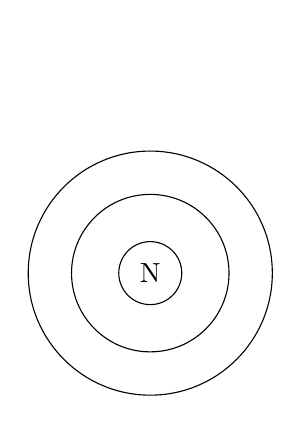
\begin{tikzpicture} 
        
        \draw(0,0) circle (0.4cm)
        node[draw=none,sloped]{};    
        
        
        \draw(0,0) circle (1cm) node[draw=none,sloped]{N};
        
        \draw(0,0) circle (1.55cm);
        \node[draw=none,align=center, font=\scriptsize,text width = 1.25cm] at (0,3) {};
        
        % \draw(0,0) circle (2.35cm);
        % \node[draw=none,align=center, font=\scriptsize,text width = 1.25cm] at (0,4) {};
        
        %   \draw(0,-9) circle (0.4cm);
        %   \node[draw=none,align=center, font=\scriptsize,text width = 1.25cm] at (0,-9) {fsgsdgf};  
        
        %   \draw(0,-9) circle (0.75cm);
        %   \node[draw=none,align=center, font=\scriptsize,text width = 1.25cm] at (0,-7.8) {fgdsfg};
        
        %   \draw(0,-9) circle (1.25cm) node[midway,sloped] at (0,-9) {dfsdfad};
        
        %   \draw(0,-9) circle (2.8cm);
        %   \node[draw=none,align=center, font=\scriptsize,text width = 1.25cm] at (0,-6.4) {dfsdfsd};
        
        %   \draw(0,-9) circle (3.2cm);
        %   \node[draw=none,align=center, font=\scriptsize,text width = 1.25cm] at (0,-6) {dfsdfsd};
        
        %   \draw(0,-9) circle (3.6cm);
        %   \node[draw=none,align=center, font=\scriptsize,text width = 1.25cm] at (0,-5.6) {sfdsfd};
        
        %   \draw(0,-9) circle (4.4cm);
        %   \node[draw=none,align=center, font=\scriptsize,text width = 1.25cm] at (0,-4.8) {sdfsf}; 
        
        %   \pgfsetlinewidth{3pt} 
        %   \draw [-implies][->] (0,-4) -- (0,-4.6);
        
        
    \end{tikzpicture} 
\end{center}
    
    \end{figure}
\end{document}